\documentclass[tikz]{standalone}

\colorlet{FilledSurface}{blue!20}
\colorlet{FilledSurfaceGroupOne}{blue!20}
\colorlet{FilledSurfaceGroupTwo}{red!20}
\colorlet{FilledSurfaceGroupThree}{green!20}
\colorlet{FilledSurfaceGroupFour}{magenta!20}
\colorlet{FormulaBackground}{green!10}
\colorlet{FormulaFrame}{green}


\usetikzlibrary{calc, decorations.markings, intersections, angles}

\tikzset{
    mark rect/.style={
        decoration={markings, mark=at position 0.5 with {
            \draw[draw=black, fill=white] (-6pt,-2pt) rectangle (6pt,2pt);
        }}, postaction={decorate}
    },
    mark rhombus/.style={
        decoration={
            markings,
            mark=at position 0.5 with {
                \draw[solid, fill=white] (0,5pt) -- (2pt,0) -- (0,-5pt) -- (-2pt,0) -- cycle;
            }
        },
        postaction={decorate}
    },
    mark one circle/.style={
        decoration={markings, mark=at position 0.5 with {
                \draw[fill=white] (0,0) circle (2pt);
        }}, postaction={decorate}
    },
    mark two circles/.style={
        decoration={markings, mark=at position 0.5 with {
                \draw[fill=white] (-2pt,0) circle (2pt);
                \draw[fill=white] (2pt,0) circle (2pt);
        }}, postaction={decorate}
    }
}

\begin{document}
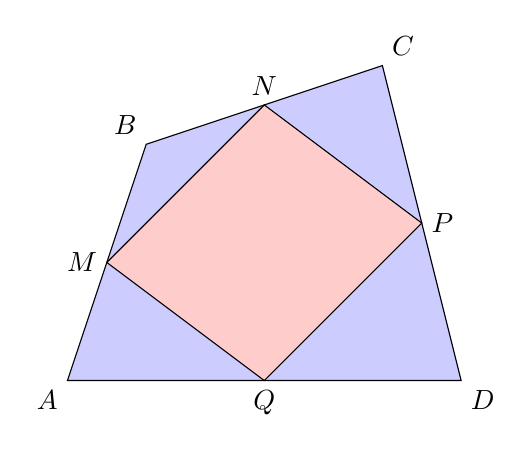
\begin{tikzpicture}

\coordinate (A) at (0, 0);
\coordinate (B) at (1, 3);
\coordinate (C) at (4, 4);
\coordinate (D) at (5, 0);

% Hallar puntos medios de cada lado del cuadrilátero.
\coordinate (M) at ($(A)!0.5!(B)$);
\coordinate (N) at ($(B)!0.5!(C)$);
\coordinate (P) at ($(C)!0.5!(D)$);
\coordinate (Q) at ($(D)!0.5!(A)$);

% Colorerar superficies
\draw[fill=FilledSurfaceGroupOne, draw=none] (A) -- (B) -- (C) -- (D) -- cycle;
\draw[fill=FilledSurfaceGroupTwo] (M) -- (N) -- (P) -- (Q) -- cycle;

% Dibujamos los segmentos, luego de colorear las superficies para
% evitar que las superficies cubran a los segmentos.

% Dibujar cuadrilátero y nombrar los vértices del cuadrilátero
\draw
    (A) node[below left]{$A$}
    -- (B) node[above left]{$B$}
    -- (C) node[above right]{$C$}
    -- (D) node[below right]{$D$}
    -- cycle;

% Dibujar medianas y nombrar los puntos medios de cada lado.
\path
   (M) node [left] {$M$}
-- (N) node [above] {$N$}
-- (P) node [right] {$P$}
-- (Q) node [below] {$Q$}
-- cycle;

\end{tikzpicture}
\end{document}
